\documentclass[sigconf]{acmart}

\usepackage{graphicx}
\usepackage{algorithm} % for algorithms
\usepackage{algpseudocode}
\algblockdefx[Process]{Process}{EndProcess}[2][Unknown]{{\bf Process} {\it #2}}{}
\algblockdefx[Event]{Event}{EndEvent}[2][Unknown]{{\bf upon event #2 do}}{}

\usepackage{booktabs} % For formal tables
%\usepackage{cite} %for multiple refs

\usepackage{amssymb} %for nice emptyset

\usepackage{amsmath}
\DeclareMathOperator{\rank}{rank}
\makeatletter
\newenvironment{sqcases}{%
  \matrix@check\sqcases\env@sqcases
}{%
  \endarray\right.%
}
\def\env@sqcases{%
  \let\@ifnextchar\new@ifnextchar
  \left\lbrack
  \def\arraystretch{1.2}%
  \array{@{}l@{\quad}l@{}}%
}
\makeatother

\usepackage{amsthm}
 
\theoremstyle{definition}
\newtheorem{definition}{Definition}
\newtheorem{corollary}{Corollary}
\newtheorem{theorem}{Theorem}

\settopmatter{printacmref=false, printccs=true, printfolios=true}
\pagestyle{plain} % removes running headers

\newcommand{\PicScale}{0.5}
\newcommand {\FlameStream} {Icetream}
\begin{document}

\title {A formalization of consistency guarantees for distributed stream processing}

% \author{  Igor E. Kuralenok,$^1$     Artem Trofimov,$^ {1,2}$    Nikita Marshalkin,$^ {1,2}$   and  Boris Novikov$^ {1,2}$ }
% \affiliation{%
% \institution{$^1$JetBrains Research}
%   \city{St. Petersburg} 
%   \country{Russia}
% }
% \affiliation{%
% \institution{$^2$Saint Petersburg State University}
%   \city{St. Petersburg} 
%   \country{Russia}
% }
% \email{\string{ikuralenok, trofimov9artem, marnikitta\string}@gmail.com, borisnov@acm.org}

% \begin{abstract}
% Currently, large-scale distributed stream processing is a hot area of research. While state-of-the-art distributed stream processing systems are able to provide low-latency under at-most-once and at-least-once guarantees, achieving exactly-once semantics is still a challenging problem. An important reason behind this fact was the lack of efficient implementation techniques for idempotent stream processing model. In this work, we apply a low-overhead deterministic model to the problem of exactly-once. We demonstrate the lightweight protocols which use the property of determinism for achieving system-wide idempotence, and, therefore, exactly-once. Our experiments show that proposed approach can significantly outperform an alternative industrial solution.
% \end{abstract}

\maketitle

\section{Preliminaries}

In this section, we remind main concepts of stream processing, which we use further in this paper. Basically, a distributed stream processing system is a shared-nothing distributed runtime, that can handle a potentially unlimited sequence of input items. Each item can be transformed multiple times before the final result is released from the system. Elements can be processed one-by-one or grouped into small input sets, usually called {\em micro-batches}. 

An element has been {\em entered} if the system is aware of this element since that moment and takes some kind of responsibility for its processing. This concept can be implemented in a different way in different systems. For example, in Flink the fact that the element has been entered means that the element has arrived at {\em Source} vertex. In Spark Streaming, element enters, when it is read or received by an input agent also called {\em Source}. 

An element has {\em left} the system if an element has been released to a consumer. Since that time system cannot observe it anymore. This concept can also be implemented differently in various systems. For instance, in Spark Streaming element leaves when it is pushed to output operation, .e.g., written to HDFS or file. In Flink element leaves when it leaves from {\em Sink} vertex.   

It is important to note that input and output elements cannot be directly matched due to a possibility of complex transformations within the system. For instance, a single input element can be transformed into multiple ones. Hence, in a general case, it is impossible to determine input element by an output.

The way how a system transforms input elements is usually defined in the form of a {\em logical graph}. A logical graph is a graph, typically set up by a user, where vertices are {\em business-logic} operations and edges determine the order of processing. Each user-defined operation may be {\em stateless} or {\em stateful}. States of operations are usually managed by the system itself to prevent inconsistencies.

The main difference between the state of user-defined operation and an ordinary element is that the state is consumed, updated, and produced by the same operation. In~\cite{we2018adbis} it is shown that operations state can practically be an ordinary data flow element for any stateful operation. Therefore, without loss of generality, we can assume that the states of operations are just special elements in a data flow.

\section {Motivation}

In state-of-the-art stream processing systems~\cite{carbone2015apache, apache:storm, Zaharia:2016:ASU:3013530.2934664} a contract with end-user regarding ~{\em which data} will be eventually processed and released in case of failures is usually described in terms of so-called~{\em delivery guarantees}. These guarantees include {\em at most once}, {\em at least once}, and {\em exactly once}. {\it At most once} states that each input event is processed once or not processed at all. {\it At least once} guarantees that each input item is processed, but possibly multiple times, that can lead to result duplication. {\it Exactly once} assures that each input event is processed exactly one time.

A tricky thing in these seemingly simple definitions is that output item depends not only on the corresponding input item but also on the {\em state} of data flow operations and on the other elements in a data flow. This fact implies that a system can {\em technically} support exactly once delivery guarantee, but in practice can release completely invalid results, because of inconsistencies in the state or in-flight elements. Another vague point is the possibility of the generation of multiple elements from one inside a data flow. If these elements are applied to state or released non-atomically, it can lead to inconsistencies as well. State-of-the-art stream processing systems avoid these types of inconsistencies using complex recovery and state management mechanisms~\cite{Carbone:2017:SMA:3137765.3137777}. In terms of these systems, exactly once or at most once is not only about delivery but is also about {\em consistency}. We believe that such meaning is much more reasonable, and further in this paper, we will call them {\em consistency guarantees}.   

However, lack of formalism in the definitions of such streaming consistency guarantees is constantly causing debates and misunderstandings~\cite{JerryPengStreamIO, PaperTrail}. There is a need to introduce formal definitions in order to describe what exactly state-of-the-art stream processing engines guarantee. Such formalisms can also help to illustrate the differences between existing approaches.

% In order to make our mathematical model independent of any implementation, we consider streaming consistency guarantees as correspondences between input and output streams and system state. If we formulate guarantees only in these terms, they can be applied to any system. However, the question of what to consider as a system state is a little bit sophisticated. At a very high-level, we can define a state as a {\em information} about input elements, which have been previously entered the system.  

% An obvious idea is to say that system state is a state of user-defined operations, i.e., so-called {\em business logic} state. The main purpose of the states of operations is to accumulate the information about input items. It allows a system to not store all previous input elements in order to process a new one in a stateful user-defined operation. However, output items can be affected not only by input ones and operations state but also by other elements, which are currently in the system. For instance, if cycles are allowed in a logical graph, cycling elements can affect output ones, but they do not belong to a state. In-flight elements can also influence the result, being not in the state. These examples demonstrate the evident fact that information about input elements can be contained not only in the states of operations but in data flow elements as well.

\section{Formalization of consistency guarantees}

\begin{definition}{Stream processing system}
is a tuple of $(\Gamma,D,W)$, where $\Gamma$ is all possible data flow elements, $D$ is dependency relation between elements, and $W$ is a set of elements in a system. 
\end{definition}

\begin{definition}{Dependency relation}
$D\subseteq{\Gamma\times\Gamma}$ is a binary relation. Pair $(x,y)\in{D}$ iff $y$ can be generated from $x$ within logical graph operations.
\end{definition}

Let $\tau\in{\mathbb{N}}$ be an exact global discrete time. Let $a_\tau\in{\Gamma}$ be the element, which enters at the time $\tau$, and $b_\tau\in{\Gamma}$ is the element, which leaves at the time $\tau$. 

\begin{definition}{Working set}
$W_\tau\subseteq{\Gamma}$ at the time $\tau$ is the set of elements, which are currently in the system:

$W_0=\emptyset$:

$W_{\tau+1}=\begin{sqcases}
W_{\tau}\cup{a_\tau}, & \text{or}\\
W_{\tau}\setminus{b_{\tau+1}}, & \text{or}\\
W_{\tau}\setminus{X}\cup{Y}, \forall{x\in{X}\exists{y\in{Y}}}:(x,y)\in{D} & \text{}.
\end{sqcases}$

\end{definition}

We can imagine a stream processing system as a pool, where some elements are poured in and others are poured out. Inside a pool, each element can be substituted by the other element, which can be substituted as well, and so on. Only survived elements are poured out from the pool.

In terms of proposed definitions, we can declare any state-of-the-art stream processing system. In Storm, $\Gamma$ contains all possible {\em Tuples}, while in Flink all {\em StreamRecords}. The notion of dependency $D$ expresses two possible scenarios. The first one is a transformation into other elements due to, e.g., {\em Bolts} in Storm or {\em Operators} in Flink. In this case, transformed elements depend on original ones. The second option is combining an element and a {\em state} into the new state. It implies that the new state depends on the previous state and the element. In both Storm and Flink, a state can be managed using state handlers, e.g., {\em KeyValueState} in Storm and {\em ValueState} in Flink. Technically, states in these systems are not data flow elements, but as it was mentioned above, they can be considered as data flow elements without loss of generality.

Regarding dependencies, we can draw an analogy with {\em Herbrand semantics}, where binary relation is used to express, which write operations affect the read operation.

Let $A_{\infty}=\bigcup\limits_{i=1}^{\infty}{a_i}$ be a set of all input elements.

\begin{definition}{User or business-logic state}
$S_\tau$ at the time $\tau$ is $W_{\infty}$ if $A_{\infty}=\bigcup\limits_{i=1}^{\tau}{a_i}$.
\end{definition}

\begin{definition}{Nullification time}
of an input element $a_\tau$ is the time $\theta_{a_\tau}=inf(\hat{\tau}>\tau|W_{\hat{\tau}}\setminus{S_{\hat{\tau}}}\cap{Cl(D)(a_\tau)=\emptyset})$, where $Cl(D)$ is a transitive closure of the relation $D$.
\end{definition}

The main purpose of user state is to accumulate the information about input items. In most systems, the user state is stored on disk or in the external system, e.g., key-value storage. It is commonly assumed that $||{W}\setminus{S}||<m<<||S||$, where $m$ is the memory size of all computational units. Hence, for each input element $a_\tau$, there must be a nullification time $\theta_{a_\tau}$, thereafter all elements, which depend on $a_\tau$, are in the user state. Otherwise, $W\setminus{S}$ will be eventually overflowed. Since the nullification time, the input element can affect output elements only through the state. The concept of nullification is shown in Figure~\ref{nullification}.   

\begin{figure}[htbp]
  \centering
  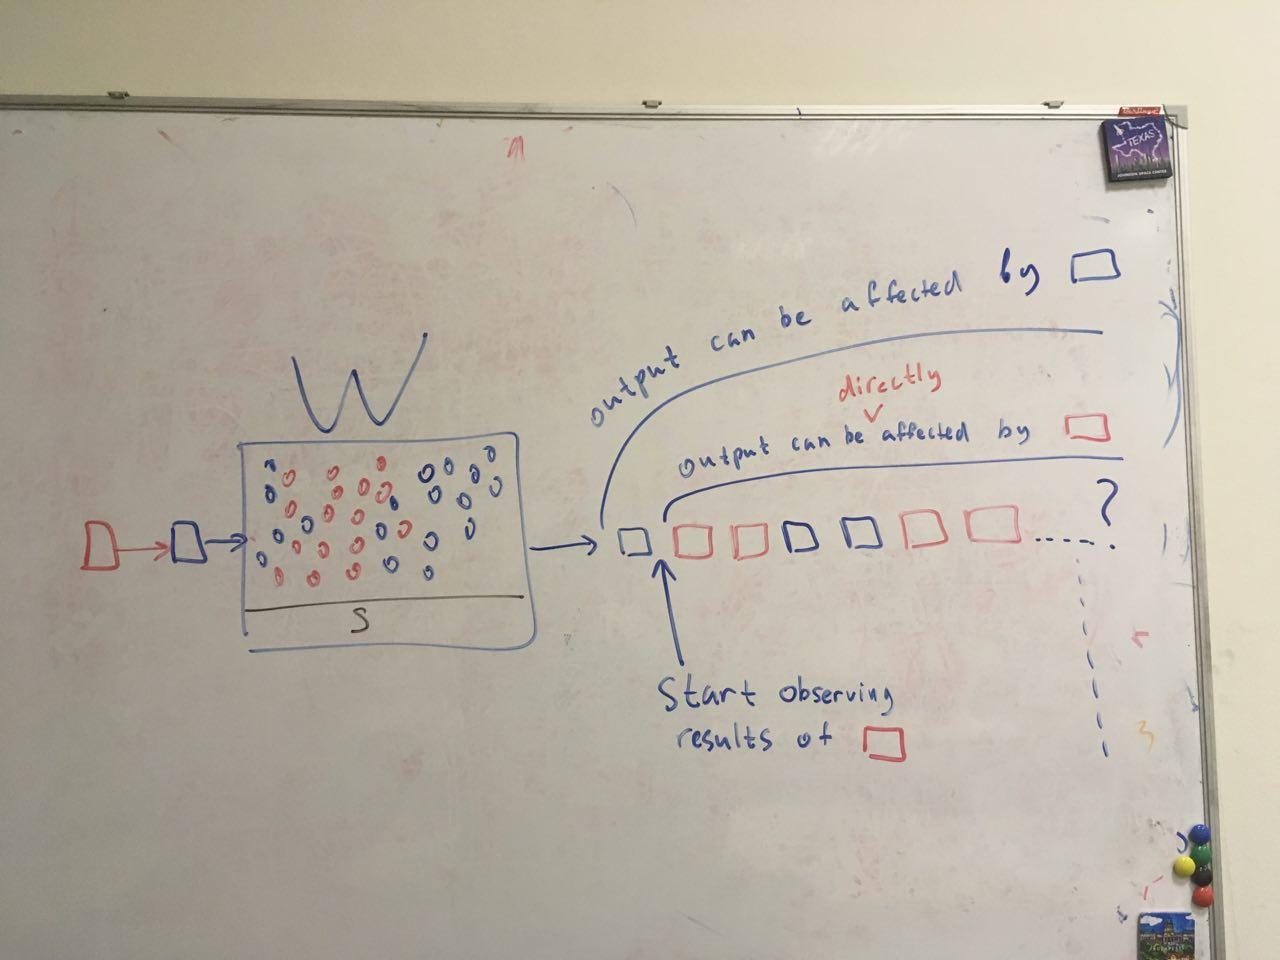
\includegraphics[width=0.48\textwidth]{pics/nullification}
  \caption{The red and blue elements have entered the system. Since that time, it is unclear, when they stop directly affect output elements}
  \label {nullification}
\end{figure}

\begin{definition}{Time quantization}
$t$ is the time of input, output, and nullification:

$t=\begin{cases}
\tau_i:\exists{a_{\tau_i}}, \\
\tau_o:\exists{b_{\tau_o}}, \\
\theta_{a_\tau}:\forall{a_\tau}.
\end{cases}$
\end{definition}

Time quantization allows us to consider only {\em observable} points in time. The time of input and output elements is obviously observed by any system. The mechanisms for tracking nullification vary slightly more. In Storm, a special agent called {\em Acker} is used. In Flink, nullification time is tracked using {\em low watermarks}. In Spark Streaming nullification time for each element in a micro-batch coincides with the time, when the micro-batch is fully processed.

Let $x,a^{1},a^\infty$ be input elements with arbitrary arrival times. $\mathbb{B}_t$ are all output elements by the time $t$:

$\mathbb{B}_t=\bigcup\limits_{i=1}^{t}{b_i}$

Let $p(W_t,\mathbb{B}_t|x,a^{1}...a^\infty)$ be a probability to observe state $W_t$ and output elements $B_t$ at the time $t$ if input elements are $x,a^{1},a^\infty$. Let us construct three sets:

$X^0=(W_\infty,\mathbb{B}_\infty|p(W_\infty,\mathbb{B}_\infty|a^{1}...a^\infty)\neq{0})$

$X^1=(W_{\theta_{x}},\mathbb{B}_{\theta_{x}}|p(W_{\theta_{x}},\mathbb{B}_{\theta_{x}}|x,a^{1}...a^\infty)\neq{0},\forall{i}:{a^i}\neq{x})$

$X^{*}=(W_{\theta_{x}},\mathbb{B}_{\theta_{x}}|p(W_{\theta_{x}},\mathbb{B}_{\theta_{x}}|x,a^{1}...a^\infty)\neq{0},\\
\exists{i}:{a^i={x}},\exists{y:y\in{W_{\theta_{x}}\setminus{S_{\theta_x}}}\cap{Cl(D)(a^i)}})$

These sets model the {\em observable} output, current elements, and state of a stream processing engine. $X^0$ expresses the case, when element $x$ has not affected the system, so it is a forbidden behavior for at least once and exactly once guarantees. On the other hand, $X^{*}$ defines possible results, after $x$ has been nullified, but $a^i=x$ or its dependencies are in the system. Such behavior can cause inconsistencies in user state due to duplicates and should not be observed if the system provides for at most once or exactly-once. Using these modeled sets now we can define guarantees.

\begin{definition}{At most once}
guarantee is provided by a system iff $\forall{x,a^{1}...a^\infty}:X^{1}\cap{X^{*}}=\emptyset$
\end{definition}

\begin{definition}{At least once}
guarantee is provided by a system iff $\forall{x,a^{1}...a^\infty}:X^{0}\cap{X^{1}}=\emptyset$
\end{definition}

\begin{definition}{Exactly once}
guarantee is provided by a system iff $\forall{x,a^{1}...a^\infty}:X^{1}\cap{X^{*}}=\emptyset \wedge X^{0}\cap{X^{1}}=\emptyset$
\end{definition}

% Now streaming consistency guarantees are defined in terms of correspondences between input, output and the system state. Custom system or user-defined semantics are not considered in this model, e.g., if the system drops all input items, it also can be claimed as supporting exactly-once. Looking from another side, our model formally describes which properties are {\em exactly} supported by state-of-the-art stream processing systems, such as Flink, Storm, Spark Streaming, Samza, MillWheel, etc, so we can discuss its properties in unified terms.

We defined streaming consistency guarantees in terms of the proposed model. This model is suitable for state-of-the-art stream processing systems, such as Flink, Storm, Spark Streaming, Samza, MillWheel, etc, so now we can discuss its properties in unified terms.

\section{Implementation properties and notes}

% In this section, we formally define some additional concepts and demonstrate a potential way to reduce latency overhead on consistency guarantees. We mainly consider exactly once, because it is the strongest guarantee, which is extremely valuable in practice.    

\begin{definition}{System failures}
are the time moments, when the system loses its working set. 
\end{definition}

Assume that the system fails at time $\tau_f$. The naive idea for recovering is to simply start processing from the very beginning, i.e., to set $W_{\tau_f+1}=\emptyset$ and to replay the whole input stream. However, storing and replaying the whole input stream is inefficient in terms of both memory and time consuming and can violate consistency guarantees.

\begin{definition}{Snapshot}
at time $\tau_s$ is persistently stored $P_{\tau_s}\subseteq{W_{\tau_s}}$ that is not lost even in case of failure.
\end{definition}

Snapshots allow a system to restart processing since defined points. One approach for taking snapshots is to save (or update) the whole $W_{\tau}$ on each $\tau$. In this case, there is no need to replay input elements, because the system can completely restore computations using only a snapshot. Google MillWheel uses this method for recovering. {\em Strong productions} mechanism allows MillWheel to preserve exactly-once guarantee for the price of persistent updates of $P_\tau=W_\tau$ on each $\tau$~\cite{Akidau:2013:MFS:2536222.2536229}.    

Another approach is to take so-called {\em state snapshots}. This kind of snapshots is considered in practice only within the time quantization $t$. It assumes that $\forall{t_s}:P_{t_s}=S_{t_s}$ and requires replay of input element. Suppose, there is a state snapshot at time $t_s$ and a system fails at time $\tau_f>t_s$. In order to recover processing, system sets $W_{\tau_f+1}=P_{t_s}$ and requests for replay elements $a$ such that $\forall{y\in{Cl(D)(a)}}:y\notin{P_{t_s}}$. The idea of taking snapshots is illustrated in Figure~\ref{snapshotting}.

\begin{definition}{Consistent state snapshot}
$P^{c}_{t_s}=S_{t_s}$ at time $t_s$ is a snapshot such that $\forall{a}\in{Cl^{-1}(D)(P^{c}_{t_s})}:\exists{\theta_a}$.
\end{definition}

\begin{theorem}
A system, that uses state snapshots for recovery, provides for at most once guarantee only if all state snapshots are consistent.  
\end{theorem}

Our notion of consistent state snapshot modifies the classical definition of {\em consistent distributed snapshot} proposed in~\cite{Chandy:1985:DSD:214451.214456} for the case where dependencies between messages exist and input element must be applied to state atomically with its inversed dependencies. This notion is natural for stream processing systems because as it was shown, it is directly connected with streaming consistency guarantees. 

One popular method for taking consistent state snapshot is to artificially reproduce a moment $t_s$, when $\forall{a}\in{Cl^{-1}(D)(S_{t_s})}:\exists{\theta_a}$, and to save obtained $S_{t_s}$. Such approach is adopted in Apache Flink~\cite{Carbone:2017:SMA:3137765.3137777} and Apache Storm~\cite{apache:storm:state}. They achieve consistent state by injecting special elements called {\em checkpoints} into the input elements. Checkpoints go through the same network channels as ordinary elements and push all inverted dependencies of inputs through the system. Each operation in data flow prepares its snapshot independently at the moment of checkpoint arriving. Global snapshot is taken when checkpoint passes through the whole data flow. 

Checkpoints cause latency overhead because they periodically block some inputs of an operation with multiple inputs. This behavior is known as {\em checkpoints alignment}. Consistent state snapshotting can be potentially relaxed if there is a mechanism to retrieve only a consistent part of each operation state at any moment in time. In this case, there is no need to technically reproduce a moment, when it is consistent, in order to obtain it.

Another property that directly affects consistency guarantees is {\em determinism}. Let $a_1...a_\infty$ be ordered in time input elements.

\begin{definition}{Data processing system is {\em deterministic}}
if \\
$\forall{t} \forall{n\geq1} \forall{a_1...a_n}\exists{\mathbb{B}_t={\{b_1...b_m\}}}:\sum\limits_{W_t} p(W_t,\mathbb{B}_t|a_1...a_n)=1$.
\end{definition}

\begin{theorem}
A non-deterministic system provides for at most once guarantee only if $\forall{b_{t_o}}:\exists{P^{c}_{t_o}} \wedge \forall{a\in{Cl^{-1}(b_{t_o})}},\theta_a=t_o$.  
\end{theorem}

Hence, non-deterministic systems that use state snapshots must atomically output elements and take a consistent snapshot that contains their inverted dependencies. In practice, it means that latency in the worst case in such systems is bounded from below by the duration of snapshotting. Besides, there is a trade-off between latency and the frequency of taking snapshots.

On the other hand, if a system is deterministic, atomicity between output and snapshotting is not necessary, because in case of replay system releases exactly the same output, that can be simply deduplicated at the very last node in a data flow. Therefore, the open questions are: is it more efficient in practice to handle non-determinism by atomic snapshotting and output or not? Can determinism be implemented in a more effective way than snapshotting?

% \section{Plan}

% 1. Определение системы: $\Gamma,D,W_\tau$.

% 2. Ванна, семантики, Spark Streaming

% 3. Пользовательский стейт и как им пользоваться. Картинка: как элементы могут идти через стейт и напрямую.

% 4. Рассуждение о накоплении информации в дополнении к пользовательскому стейту. Противоречие. Как следствие, моменты дырок.

% 5. Квантизация и наблюдение за дырками. Отсутсвие активности и лоу вотермарки. Перешли от непонятного времени к наблюдаемому.

% 8. Теперь давайте определим гарантии. ИКСЫ + Гарантии.

% % 9. Это были гарантии доставки?

% 6. Все было бы круто и легко, но система может падать. Не хотим идти с начала. Иначе - батчинг. Снепшот - можем сохранить $W_\tau$. 

% 7. Для этого либо "сдуть", либо как есть. Сдуть значит остановить вход до момента, пока $W_\tau=S_\tau$. По этому пути идут все. По другому -  MillWheel.

% 5. Рассуждение о том, как дырки соотносятся с выходными элементами. Дырки не могут образовываться до выхода. Только полсе или совместно. Вред от того, если дырка образуется после выхода.

% 7. Если дырки образуются после выхода элемента, то есть элементы, которые не попали в снепшот. Теорема. 

% Давайте разберем несколько практических реализаций

\bibliographystyle{ACM-Reference-Format}
\bibliography{../../bibliography/flame-stream.bib}
\end {document}

\endinput
you can put whatever here
